% Hoveddel

\chapter{Hoveddel} % Chapter title

\label{ch:hoveddel} % For referencing the chapter elsewhere, use \autoref{ch:mathtest}

%----------------------------------------------------------------------------------------

% Skrives i fortid.

\todo{Passe på alle seksjonene i hoveddelen følger det som forventes: Gjengi situasjoner med forbedringspotensial. Referanse til teori som kaster lys over utfordringen. Reflektere over svakheter og hvordan vi kan forbedre oss, kombinert med teori. Evaluere om målene ble nådd.}
\todo{Generelt bør det trekkes mer teori inn i hoveddelen. Enten som forklarer hvorfor en situasjon / handling har skjedd eller ikke skjedd, eller som beskriver hva som kunne vært gjort bedre eller annerledes eller om noe var riktig.}

Siden gruppen ikke har gjennomgått noen store eller viktige situasjoner som har hatt mye innvirkning, velger vi heller å fokusere på mange små hendelser som har vært med på å forme utviklingen av samarbeidet i gruppen.


\section{Effektivitet og ytelse}


Allerede fra første dag har det vært et fokus på å holde høy effektivitet innad i gruppen, slik at jobbing utenom onsdager ble ungått. Dette ble også formalisert som et eget punkt i kontrakten som gruppen skrev i starten av perioden. I starten, når det var mye diskusjon, ble det ofte en del avsporing og tulling. For å øke effektiviteten i gruppen satte vi ofte tidsfrister på dette slik at det var greit å være litt useriøs, men for eksempel kun to minutter til. Litt tulling bidrar til god gruppefølelse og gir rom for en mer avslappet atmosfære. Derfor var det ikke utelukkende negativt at dette fant sted, spesielt i startfasen. 

Noen medlemmer av gruppen hadde erfaring fra arbeidslivet, og en del effektiviseringsteknikker ble derfor hentet derfra. I begynnelsen ble blant annet Scrum tatt i bruk. Såkalte <<Stand-up>>-møter har også blitt benyttet av gruppen. Dette er korte morgenmøter hvor hvert medlem forteller om hva som ble gjort forrige gang, og hva som skal gjøres for dagen. Morgenmøtene har bidratt til å iverksette medlemmene på gruppen, og effektivt sørget for at hvert medlem til enhver tid har hatt noe å gjøre.

Flere i gruppen brukte mye tid på å sette seg inn i ulike stifinnings\-algoritmer for så å finne ut at systemet allerede hadde funksjoner som støttet dette. Dette var ikke på grunn av en kommunikasjonssvikt, men kunne vært unngått om vi hadde en person som bedre kjente til funksjonene til roboten. Denne hendelsen førte til tapt tid for gruppen og nedsatt motivasjon for dem som hadde brukt tid på arbeid som det ikke var behov for likevel. 

En av hovedårsakene til nedsatt effektivitet i gruppen var at kun én datamaskin kunne kommunisere med roboten. Dette begrenset mengden med teknisk arbeid som kunne utføres samtidig. Det finnes et simuleringsverktøy som kunne fjernet flaskehalsen, dette ville helt klart økt effektiviteten på sikt, men man ville brukt mye tid på å sette seg inn i dette. Med tanke på at prosjektetperioden var så kort ville det trolig ikke vært lønnsomt i vårt tilfelle. Gruppen kom derfor frem til at simuleringsverktøyet skulle nedprioriteres.

I løpet av arbeidsperioden som gruppen har vært gjennom, har det vært tydelig at engasjement og moral er en viktig faktor for effektivitet. En kunne observere en klar nedgang i effektiviteten ettersom gruppen ble nødt til å endre kurs som en følge av råd fra veileder.  

\section{Kommunikasjon}
I gruppen vår hadde vi alle bakgrunner fra tekniske studieretninger, vi unngikk derfor de største utfordringene rundt tverrfaglig kommunikasjon. Likevel hadde vi et tilfelle i oppstartfasen hvor en spesifikk tekniske løsning ble diskutert i gruppen på et så detaljert plan at kun noen få av gruppens medlemmer klarte å henge med. Det ble laget et sosiogram av samtalen i gruppen på dette tidspunktet og resultatet kan sees i \autoref{sosiogram}.

\begin{figure}[!ht]
    \centering
    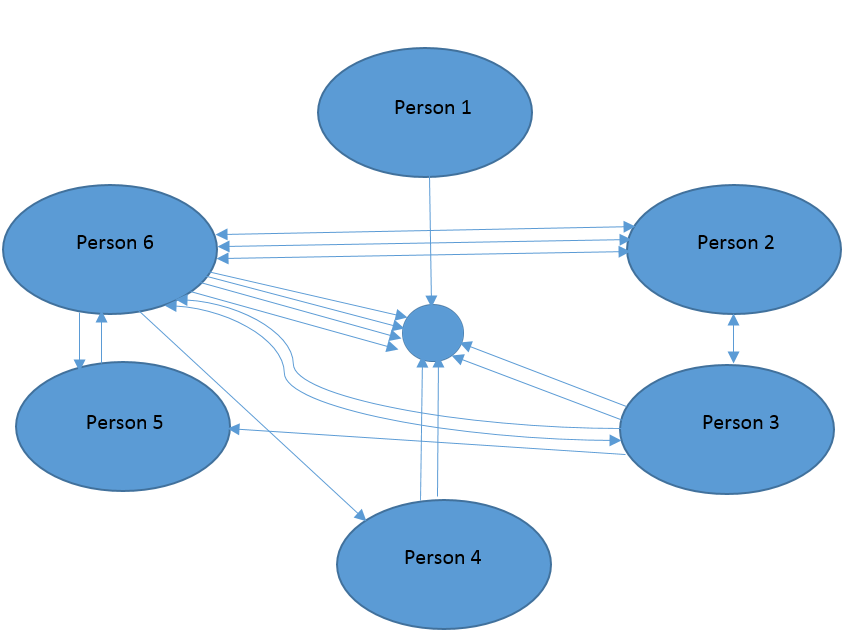
\includegraphics[scale=0.7]{gfx/sosiogram1.PNG}
    \caption{Sosiogram}
    \label{sosiogram}
\end{figure}

Person 2 og Person 6 hadde begge bakgrunn innen temaet som ble diskutert og samtalen gikk derfor mye mellom dem, mens resten hørte på. Vi kom i ettertid frem til at dette var en lite effektiv måte å jobbe på. Det ble derfor bestemt at diskusjoner som gikk på detaljnivå og hvor hele gruppens meninger ikke var nødvendig, skulle taes opp i mindre subgrupper mellom dem det gjaldt. På denne måten fikk vi bedret gruppens effektivitet og i tillegg utnyttet de ulike gruppemedlemmenes kompetanse på en bedre måte. 

\section{Gjennomføring av kreative prosesser}
De kreative prosessene i gruppen begynte i hovedsak da vi skulle velge oppgave å jobbe med. Vi brukte brainstorming til å komme frem til de fleste idéene våre. Med litt god tid til denne prosessen kom det frem mange forslag og alle fikk ytret sine meninger. Gjen\-tatte ganger ble forslag til problemstilling ikke godkjent av landsbyhøvding på grunn av simpel idé, lite realistisk eller gjennomførbar oppgave, eller problemstilling for lite relatert til robot. 

Den tredje landsbydagen måtte gruppen komme opp med en ny problemstilling siden daværende problemstilling ble litt for simpel. Flere reagerte negativt og ble litt skuffet siden de var motivert for idéen gruppen måtte bevege seg bort fra. Utfordringen her var å endre problemstillingen slik at alle gruppemedlemmene ble like fornøyd. Det hadde vært nok arbeid å komme frem til problemstillingen gruppen hadde bestemt seg for. To av gruppemedlemmene var forberedt på at gruppen kanskje måtte velge ny problemstilling, dermed hadde de litt mer positiv innstilling. Dette hjalp resten av gruppen med å komme seg videre og bli fornøyd med en ny problemstilling. 

\section{Rollebevissthet og fleksibilitet i rollevalg}
I gruppen er det et medlem som har driftet mot en lederrolle, særlig når gruppen har vært lite motivert. Denne personen påvirker gruppen med sitt fravær, eller tilstedeværelse. Gruppen har merket ved flere anledninger hvor han enten har vært borte en liten del eller hele dagen, at effektiviteten kan gå litt ned. Denne personen har hele tiden aktivt søkt tilbakemelding for å få vite hva resten av gruppen syntes om måten han ledet på og i hvilke situasjoner han tredde inn i rollen. 


\section{Effektiv beslutningstaking}
I løpet av idéfasen fant et av gruppemedlemmene ut at metoden som var planlagt å bruke for å finne posisjon eller avstand ikke var mulig for oss å implementere. Han var dermed allerede innstilt på at vi måtte endre på idéen vår når han møtte opp den dagen, noe resten av gruppen ikke var. For å få litt fortgang på arbeidet la han press på gruppen til å ta et valg, og ville ha en håndsopprekning for å avgjøre det videre arbeidet. En annen på gruppen følte at han ikke hadde fått nok tid og sa ifra. Dermed tok gruppen en pause og fikk bedre tid til å bestemme seg. Denne betenkningstiden gjorde at vi endte opp med en helt ny idé. Denne nye idéen ble grunnlaget til prosjektet sånn det endte opp. Etter at gruppen fikk oppleve hvor stor forskjell ordentlig betenkningstid kan gjøre, ble vi veldig oppmerksom på å ha nok tid før viktige avgjørelser. Om vi visste at en avgjørelse måtte bli tatt ved neste landsbydag gjorde vi det til en vane å ta opp saken på slutten av dagen, slik at vi kunne tenke på det til gangen etter.
    
Gruppen skulle på et tidspunkt avgjøre om kamerasystemet skulle brukes eller ikke. Et av gruppemedlemmene, som hadde litt mer oversikt enn andre, presenterte både for- og motargumenter for begge scenarioene. Selv om han hadde gjort seg opp en menig allerede, la han frem argumentene på en objektiv måte og forsikret gruppen om at han ville respektere flertallets avgjørelse uansett. Resten av gruppen syntes dette var en veldig ryddig og fin måte å gjøre det på og gjorde det lettere å ta en avgjørelse.

Gruppen har hele tiden vært enig om at for å bli så effektive som mulig var det viktig at alle følte eierskap til problemstillingen. Vi var derfor nøye med å, med jevne mellomrom, gjennom hele prosessen, spørre i felleskap om alle var komfortable med retningen vi beveget oss i. 